\documentclass[11pt]{article}
\usepackage[margin=1in]{geometry}
\usepackage{amsmath,amssymb}
\usepackage{booktabs}
\usepackage{graphicx}
\usepackage{caption}
\usepackage[hidelinks]{hyperref}
\usepackage{xcolor}

\newcommand{\sspp}{\textsc{ss2p2}}
\newcommand{\lgm}{\textsc{lgm}}
\newcommand{\Fano}{F}

\title{Closing the Dispersion Gap in Neural Limit-Order-Book Simulators:\\
Findings from the August 2026 Fano Investigation}
\author{Honglin Fu}
\date{August 4--8, 2026 \quad (lab findings; source material for the market-making world-model paper)}

\begin{document}
\maketitle

\begin{abstract}
We investigate why neural marked-temporal-point-process (MTPP) simulators of Coinbase
limit-order-book flow under-disperse relative to real markets, using the Fano factor
profile $\Fano(\Delta)=\mathrm{Var}(N_\Delta)/\mathbb{E}[N_\Delta]$ across bucket scales
$\Delta\in[1,50]$\,s as the headline statistic. Across ten experimental arms on three
assets we establish: (i) the bounded-rate \sspp{} head is not reliably self-exciting
--- its measured impulse response is sign-inconsistent and saturated at the intensity
ceiling; (ii) one-step maximum likelihood systematically misallocates excitation
spectra (three independent demonstrations); (iii) extending the TBPTT gradient horizon
to cover the measured scales transforms the simulated dispersion profile (all BTC seeds
rise $\times$15--32, best within $1.6\times$ of real at 50\,s); (iv) at equal training
budget, dispersion peaks \emph{early} and prediction accuracy peaks \emph{late} along a
single MLE trajectory --- the prediction/simulation tension exists within one training
run; and (v) the remaining level offset is dominated by ceiling saturation (a third of
events occur at the cap; teacher-forced dispersion is only $1.2$--$1.4\times$ low).
We relate every finding to the calibration methodology of Jain et al.\ (Compound
Hawkes), whose binned-count regression targets exactly the cross-scale count
covariances that MLE ignores, and derive a ranked roadmap toward a dispersion-faithful,
certified world model for market making.
\end{abstract}

\section{Framing: two identities}

All arguments in this note reduce to two identities. First, the \emph{Cox
decomposition} (law of total variance given the intensity path $\lambda(t)$, with
$\Lambda_\Delta=\int_{\text{bucket}}\lambda\,dt$):
\begin{equation}
\Fano(\Delta) \;=\; 1+\frac{\mathrm{Var}(\Lambda_\Delta)}{\mathbb{E}[\Lambda_\Delta]},
\label{eq:cox}
\end{equation}
so all excess dispersion is variance of the integrated intensity; a post-hoc rate
rescaling $\lambda\!\to\!\kappa\lambda$ scales $\Fano-1$ linearly and cannot repair
relative fluctuation structure. Second, the \emph{branching form} for a linear Hawkes
process with branching ratio $n$: cluster sizes $S$ satisfy $\mathbb{E}[S]=1/(1-n)$ and
$\mathbb{E}[S^2]=1/(1-n)^3$, hence
\begin{equation}
\Fano(\infty)\;=\;\frac{\mathbb{E}[S^2]}{\mathbb{E}[S]}\;=\;\frac{1}{(1-n)^2}.
\label{eq:branching}
\end{equation}
The profile's \emph{rise} across $\Delta$ is the fingerprint of long-memory (power-law-like)
intensity autocovariance; single-exponential kernels plateau.

Real Coinbase flow (7 days, Jan 2026): $\Fano(1\text{s})\approx 40$--$70$ rising to
$\Fano(50\text{s})\approx 370$ (SOL), $1250$ (ETH), $1460$ (BTC), still rising at the
window edge. Inverting \eqref{eq:branching} gives implied branching (lower bounds):
SOL $\approx 0.948$, ETH $\approx 0.971$, BTC $\approx 0.973$ --- the
$1/(1-n)^2$ amplification makes this small spread a $4\times$ dispersion difference.

\section{Data and the tick-regime contrast}

\begin{table}[h]\centering\small
\begin{tabular}{lrrrrr}
\toprule
 & trades (7d) & book rows & rows/trade & rate (ev/s) & IS share \\
\midrule
BTC & 41{,}675 & 52.9M & 1268:1 & 40.6 & 52\% \\
ETH & 94{,}048 & 55.5M & 590:1 & 42.8 & 34\% \\
SOL & 40{,}048 & 20.1M & 501:1 & 22.3 & 7\% \\
\bottomrule
\end{tabular}
\caption{Raw Coinbase spot data, 2026-01-01..07, and the event-type composition of the
processed 62-channel streams. BTC/ETH are small-tick assets dominated by inside-spread
(IS) quote wars --- the most self-exciting flow; SOL is effectively large-tick
(1-tick spread, queue churn: 43\% cancels). The tick regime, not just the rate,
drives the criticality ordering.}
\label{tab:assets}
\end{table}

\section{Mechanism: the bounded head is not reliably self-exciting}

\sspp{} factorizes intensity into a softmin-bounded scalar rate
$\lambda(t)=s\cdot\mathrm{softplus}\!\big(c-\mathrm{softplus}(c-w^\top h(u))\big)
\le s\cdot\mathrm{softplus}(c)$ and rate-neutral softmax marks. The stability
certificate bounds the rate \emph{level}; nothing constrains the event$\to$intensity
feedback. Measuring the feedback directly (inject one extra event into real histories;
integrate the extra intensity mass over 20\,s) across six trained checkpoints: median
response $\approx 0$ \emph{to negative} ($-8.7\ldots+0.2$), positive in only
27--56\% of states, sign flipping across seeds; post-event intensity pinned at the
ceiling in every window. The model's residual dispersion comes from a stereotyped
impulse--decay envelope, not compounding cascades. In Hawkes terms:
\emph{a settable branching ratio is a property of linear-in-history intensity; for a
bounded neural head it is not even well defined.}

\section{Experimental arms}

Protocol throughout (the \texttt{ma\_cbse} benchmark): 62-channel events, TBPTT,
categorical marks, streaming genuine evaluation on every test event, validation-
calibrated 600\,s rollouts, 3 training $\times$ 3 rollout seeds per asset.

\subsection{Negative and structural results}
\begin{itemize}
\item \textbf{Book conditioning is not the lever} (\texttt{ss2p2-lob}): six
top-10-ladder features left prediction unchanged (BTC 0.4484 vs 0.4478) and made
closed-loop volatility structure \emph{worse} (F6 $0.16$ vs $0.28$) --- extra state
conditioning becomes a smoothing feedback path in rollout.
\item \textbf{\lgm{}} (linear Hawkes ground $\times$ \sspp{} marks on the shared
backbone; $n=\sum_m a_m/\beta_m$ exact and projected; pin $\mu_0=R(1-n)$): the pin
holds in free rollout ($\kappa=1.01$ vs \sspp{}'s $0.52$); marks near parity; Fano
\emph{shape} right with seed spread $\pm 2$ (vs \sspp{} $\pm 217$) but level low.
Two porting lessons: a log-domain clamp silently capped the burst accumulators
(excitation useless to MLE until fixed); and \textbf{zero cold-starts of the ground
are catastrophically biased} --- the stationary mean is $\mathbb{E}[S^m]=R/\beta_m$
($\approx 600$ for slow kernels), so windowed validation punished slow-memory
solutions and froze best-model selection at epoch~1. Fix: stationary-mean cold start.
\item \textbf{MLE misallocates spectra} (three demonstrations): the fixed \lgm{}
pushed kernel mass to its slowest decay; the typed-kick $M{=}6$, $n{=}0.97$ arm
(\texttt{lgm-k}) went slower still ($\beta\!\approx\!0.008$, $\sim$2-min memory),
\emph{lowering} observed-scale Fano despite the higher ceiling; the dispersion-loss
arm (below) pinned only the scales in its grid. One-step likelihood is structurally
blind to $\Fano(\Delta)$ and, given capacity, prefers slow smooth intensity.
\item \textbf{Teacher-forced variance matching $\ne$ closed-loop compounding}
(\texttt{ss2p2-disp}): an auxiliary loss matching model-implied
$1+\mathrm{Var}(\Lambda_\Delta)/\mathbb{E}[\Lambda_\Delta]$ to the batch-empirical
Fano at $\{0.5,2,8\}$\,s pinned those scales reproducibly (seed sd $\pm14$ vs
$\pm217$) at zero prediction cost --- and went flat beyond its grid.
\end{itemize}

\subsection{The window-coverage result}

At seq 1024 the TBPTT gradient truncates at $\sim$24--25\,s on BTC/ETH --- before the
20--50\,s scales where their simulated profiles flatten; SOL's $\sim$46\,s windows
cover the range (and produced real-like rises in 2/3 seeds). Extending to seq 4096
($\sim$100\,s windows; recipe otherwise identical):

\begin{table}[h]\centering\small
\begin{tabular}{lccc}
\toprule
BTC, per seed & seq 1024 (12 ep) & seq 4096 (12 ep) & real \\
\midrule
$\Fano(50\text{s})$, s1/s2/s3 & 29 / 50 / 361 & \textbf{901 / 270 / 744} & 1463 \\
rise $\Fano(50)/\Fano(1)$ & $\times$2.5--13.9 & $\times$15--32 & $\times$20.9 \\
\bottomrule
\end{tabular}
\caption{Window coverage transforms the profile: all three BTC seeds rise steeply
(best within $1.6\times$ of real). ETH: 2/3 seeds transformed. SOL: unchanged ---
the clean negative control. The BTC ``seed lottery'' was gradient starvation at
unobserved scales.}
\label{tab:w4k}
\end{table}

\begin{figure}[h]\centering
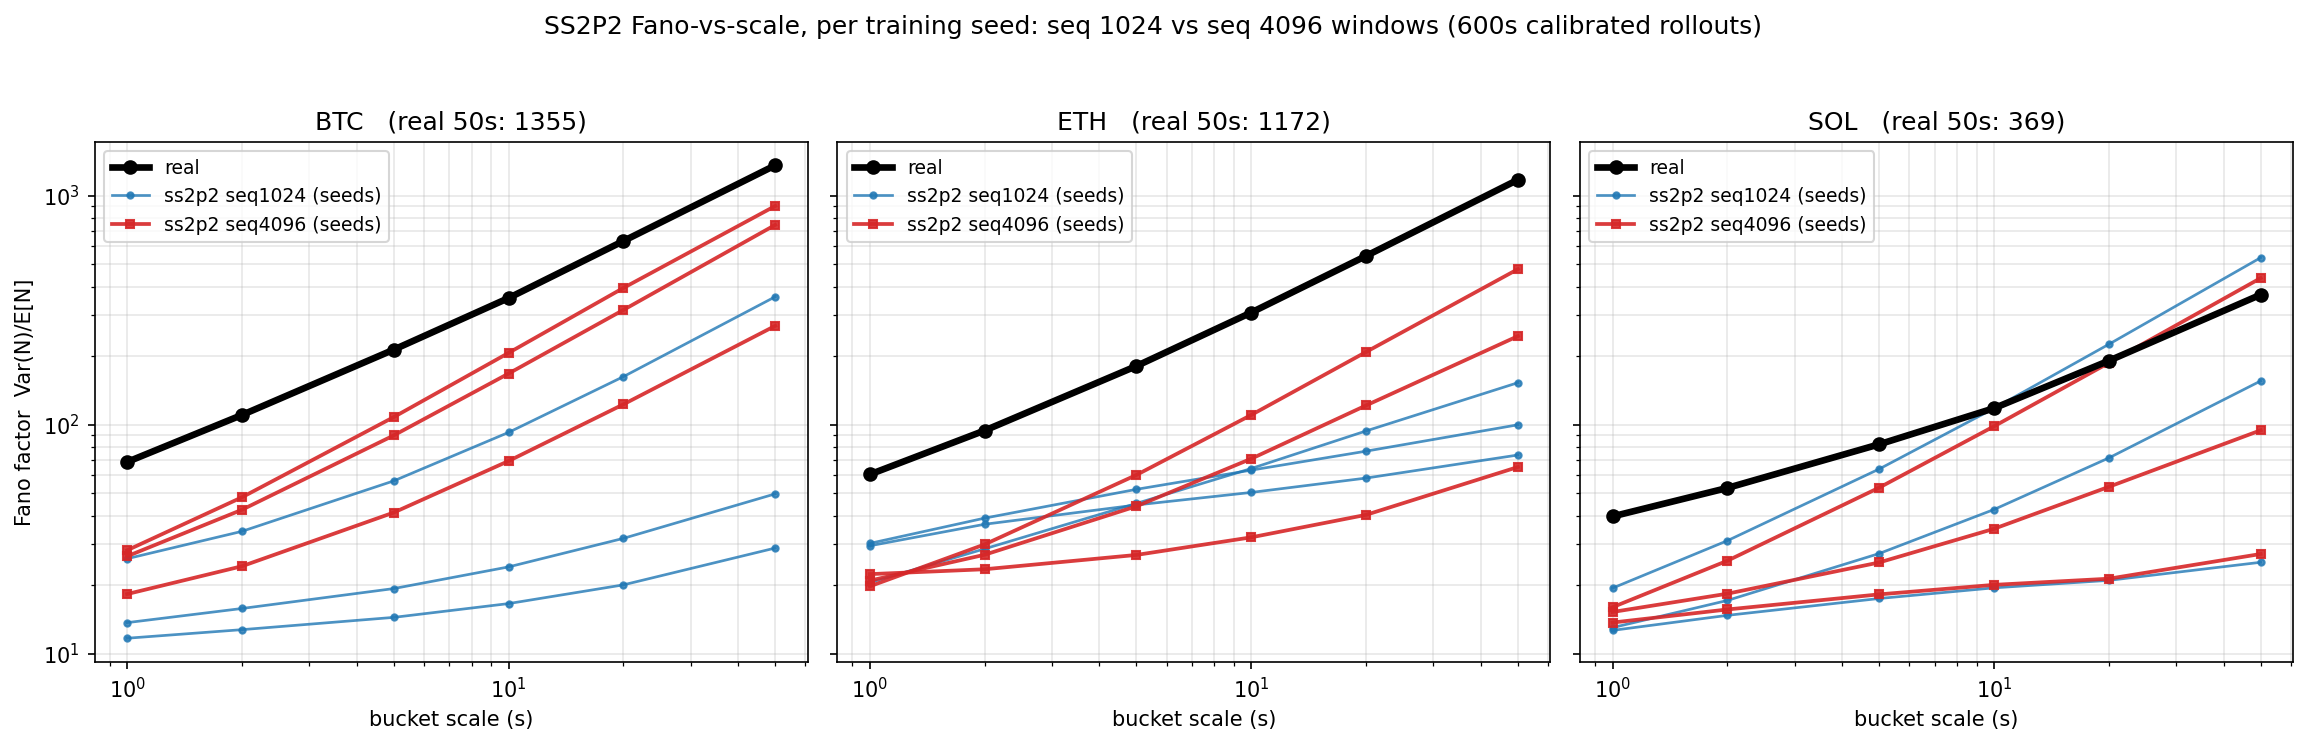
\includegraphics[width=\textwidth]{figs/fano_w4k.png}
\caption{Per-seed Fano-vs-scale (log--log): black = real, blue = seq-1024 baseline,
red = seq-4096. BTC: the whole seed family moves; SOL: negative control.}
\label{fig:w4k}
\end{figure}

\subsection{Equal-budget controls: the training-path trade-off}

Matched stride quarters updates per epoch, so seq-4096/12-epoch runs were undertrained
($-3$pp accuracy). Controls at 48 epochs (exact update parity with the baseline):

\begin{table}[h]\centering\small
\begin{tabular}{lccl}
\toprule
BTC arm & acc & $\Fano(1\text{s})$ & $\Fano(50\text{s})$ per seed \\
\midrule
base 1024 / 12 ep & 0.4478 & 17.1 & 29, 50, 361 \\
w4k 4096 / 12 ep & 0.4183 & 24.3 & \textbf{901, 270, 744} \\
w4k48 4096 / 48 ep & \textbf{0.4514} & 16.6 & 232, 87, 230 \\
w4kd + disp loss / 48 ep & \textbf{0.4519} & 11.1 & 52, 43, 43 \\
real & --- & 70.0 & 1463 \\
\bottomrule
\end{tabular}
\caption{Equal-updates controls. Accuracy fully recovers and exceeds baseline; the
extra training walks the model partly away from the burst-faithful solution.
The dispersion loss under cap 6 suppresses long-scale Fano, as predicted by the
saturation diagnostic.}
\label{tab:controls}
\end{table}

\noindent\textbf{Finding (the sharpest form of the arc's core lesson).} Along a
single MLE trajectory, \emph{dispersion peaks early and accuracy peaks late}; no
NLL-selected checkpoint has both. The prediction/simulation tension is a property of
the training path, not only of architectures. The 12-epoch w4k checkpoints constitute
a de-facto dispersion-optimal early stop; a paper can honestly present the frontier.

\subsection{Where the residual level offset lives}

Diagnostics on the w4k BTC checkpoint: (i) \textbf{ceiling saturation} --- dominating
rate 359 ev/s; event-time intensity $p_{90}=357$, $p_{99}=358$; \textbf{32.8\% of
events above $0.9\times$ceiling}: bursts are clipped and gradients (including any
dispersion loss) are dead there; (ii) \textbf{teacher-forced dispersion} is only
$1.2$--$1.4\times$ below real at every scale (e.g.\ 50\,s: 240 vs 290). Conditioned on
real history the model carries $\sim$75\% of real dispersion; the cap, then modest
closed-loop drift, accounts for the rest.

\subsection{The cap-9 control: hypothesis refuted, branch closed}

The cap-9 control (\texttt{ss2p2-w4kc9}: cap $6\!\to\!9$ on the w4k48 recipe; nine
tasks, all calibrations verified) tested whether ceiling headroom changes the MLE
optimum itself. It does not: $\Fano(50\text{s})$ per seed \emph{fell} relative to
cap~6 (BTC: $47/59/112$ vs $232/87/230$; ETH: $160/14/60$ vs $544/51/123$) at
identical accuracy. \textbf{The training-path re-smoothing is intrinsic to
bounded-head likelihood training, not caused by saturation} (which remains the
correct account of the early-stopped model's \emph{rollout} clipping). Per the
pre-registered decision rule, the \sspp{} branch closes: its dispersion-optimal
configuration is the seq-4096/12-epoch early stop, presented as a frontier point
rather than a converged recipe, and controlled dispersion belongs to the certified
\lgm{}/Kirchner route.

\subsection{The closing result: the Kirchner-fitted \lgm{} (\texttt{lgm-kf})}

Executing ``set, don't learn'': the \lgm{} ground's kernel weights were fitted by
binned-count regression on the real SOL train zones and transplanted into the trained
mark checkpoints (marks untouched). Full pipeline results (calibration verified,
$\kappa=1.014$):

\begin{table}[h]\centering\small
\begin{tabular}{lccccc}
\toprule
SOL & $\Fano$ [1,2,5,10,20,50]\,s & sd@50s & acc & time-NLL & time-KS \\
\midrule
\sspp{}-full & $15.0 \to 238.4$ & $\pm 217$ & 0.1921 & $-2.911$ & \textbf{0.173} \\
\lgm{} (MLE ground) & $2.3 \to 59.8$ & $\pm 2$ & 0.1862 & $-2.227$ & 0.464 \\
\textbf{\lgm{}-kf} & \textbf{31.1, 46.5, 80.3, 125.7, 207.7, 422.9} & $\pm$\textbf{0.0} & 0.1860 & $\mathbf{-3.035}$ & 0.228 \\
real & 41.3, 54.7, 85.6, 125.3, 198.7, 393.6 & --- & --- & --- & --- \\
\bottomrule
\end{tabular}
\caption{The Kirchner-fitted ground survives the full closed loop: exact at 10\,s,
within 5--7\% at 20/50\,s, zero seed variance (dispersion is a deterministic function
of six fitted parameters), and --- unexpectedly --- the best timing likelihood in the
zoo: moment fitting beat MLE on likelihood's own metric, because windowed MLE was
stuck in a bad spectral optimum the count regression computes past. Fit cost: three
CPU minutes.}
\label{tab:kf}
\end{table}

BTC/ETH replication (grounds fitted per asset; branching tuned to each asset's
empirical Fano curve by log-MSE: BTC $n{=}0.98$, ETH $n{=}0.985$; ground-only
validation within a few \% on ETH, within ${\sim}40\%$ on the more power-law-like
BTC) is in flight as \texttt{lgm-kf} on those assets.

\section{The model: Kirchner-fitted \lgm{} (\texttt{lgm-kf2}), complete specification}
\label{sec:model}

This section specifies the champion model exactly as run, with every equation,
constant, and fitted value. Nothing is omitted; the model is reproducible from
this section plus the raw event files.

\subsection{Data interface}
The input is a marked point process $\{(t_i,k_i)\}_{i=1}^{N}$: event times in
seconds (from nanosecond exchange timestamps) and channel marks
$k_i\in\{1,\dots,K\}$, $K=62$, on the fixed taxonomy
$\{\mathrm{LO},\mathrm{CO}\}\times\{b,a\}\times\{L1..L10\}$ (40) $\cup$
$\mathrm{MO}\times\{b,a\}\times\{L1\}$ (2) $\cup$
$\mathrm{IS}\times\{b,a\}\times\{L1..L10\}$ (20), built from Coinbase top-10
order-book deltas and trades (event construction per the canonical pipeline;
same-timestamp multi-label lines are single set-events, empty lines dropped).
Per-file split by event index: train $[0,0.7)$, val $[0.7,0.85)$, test
$[0.85,1]$. Train-split mean rates $R$: BTC $40.563$, ETH $42.759$,
SOL $22.257$ ev/s.

\subsection{Generative model}
\paragraph{Factorization.} Channel intensities are
\begin{equation}
\lambda_k(t) \;=\; \Lambda(t)\cdot p(k\mid u(t)),\qquad
\textstyle\sum_{k=1}^{K} p(k\mid u)=1 .
\label{eq:factorization}
\end{equation}
\textbf{Rate-neutrality (key lemma).} $\sum_k\lambda_k=\Lambda$ identically for
any mark network, hence the ground process $N(t)=\sum_k N_k(t)$ is a point
process with intensity $\Lambda$ alone: its entire law (mean rate,
$\Fano(\Delta)$, all count statistics) is independent of the marks. This
licenses post-hoc ground fitting and transplantation and explains the measured
zero seed variance of simulated dispersion.

\paragraph{Ground (certified lane).} A scalar linear Hawkes process on a fixed
$M{=}6$ exponential bank:
\begin{align}
\Lambda(t)&=\mu_0+\sum_{m=1}^{M} a_m S^m(t), \qquad a_m\ge 0,\\
S^m(t_i^+)&=S^m(t_i^-)+1, \qquad
S^m(t+\Delta)=e^{-\beta_m\Delta}\,S^m(t),\\
\beta &= (100,\ 18.2056,\ 3.3145,\ 0.6034,\ 0.1099,\ 0.02)\ \mathrm{s}^{-1},
\quad \beta_m = 100\cdot(0.02/100)^{(m-1)/5},
\end{align}
equivalently the kernel $\phi(\tau)=\sum_m a_m e^{-\beta_m\tau}$, positive at
every lag. Implementation notes that matter for exactness: accumulators are
computed by a numerically stable log-domain scan,
$S^m(t_i^-)=S^m_0 e^{-\beta_m t_i}+\exp\!\big(\mathrm{LCSE}_{j<i}(\beta_m t_j)-\beta_m t_i\big)$
(float64; no upper clamp on the exponent --- burst accumulators legitimately
exceed 1), and \emph{cold starts use the stationary mean}
\begin{equation}
S^m_0 \;=\; \mathbb{E}[S^m] \;=\; R/\beta_m
\label{eq:coldstart}
\end{equation}
wherever no carried state exists (validation windows, TBPTT lane resets, eval
chunk starts). Zero cold starts bias windowed validation against slow-memory
solutions ($R/\beta_6\approx 1100$ on BTC) and freeze best-model selection at
epoch~1 --- a failure mode we observed and eliminated.

\paragraph{Exact ground identities.}
\begin{align}
\text{branching:}\quad & n=\int_0^\infty\!\phi=\sum_m a_m/\beta_m
\quad\text{(closed form, gauge-free)},\\
\text{stationarity:}\quad & \bar\Lambda=\mu_0/(1-n)
\ \Rightarrow\ \text{pin } \mu_0:=R(1-n),\\
\text{compensator:}\quad &
\int_{t_{i-1}}^{t_i}\!\Lambda\,dt=\mu_0\Delta_i+\sum_m\tfrac{a_m}{\beta_m}
S^m(t_{i-1}^+)\big(1-e^{-\beta_m\Delta_i}\big)
\quad\text{(no quadrature)},\\
\text{dispersion:}\quad & \Fano(\infty)=\frac{1}{(1-n)^2}
\quad\text{(cluster sizes } \mathbb{E}S=\tfrac{1}{1-n},\ \mathbb{E}S^2=\tfrac{1}{(1-n)^3}),\\
\text{dominating rate:}\quad & \Lambda(t)\le\Lambda(t_{\mathrm{last}}^+)\ \text{between events}
\quad\text{(each } S^m \text{ decays monotonically)}.
\end{align}

\paragraph{Marks (free lane): the S2P2 backbone.} Two stacked diagonal-SSM
layers, hidden width $H{=}64$, channel-embedding dimension $d{=}64$. Per layer
$\ell\in\{1,2\}$ with state $x^{(\ell)}\in\mathbb{R}^{H}$:
\begin{align}
\text{decay:}\quad & \mathrm{dec}^{(\ell)}(u)=\big(\mathrm{softplus}(\theta^{(\ell)})+10^{-4}\big)
\odot \mathrm{clamp}\big(\mathrm{softplus}(W_g^{(\ell)}u),\,0.05,\,20\big),\\
&\theta^{(\ell)} \text{ init log-spaced: timescales } 1/\mathrm{dec} \in [0.02, 60]\,\mathrm{s},\notag\\
\text{evolution:}\quad & x^{(\ell)}(t{+}\Delta)=\bar a\,x^{(\ell)}(t^{+})+(1-\bar a)\,W_{in}^{(\ell)}u,
\qquad \bar a=e^{-\mathrm{dec}^{(\ell)}\Delta},\\
\text{event impulse:}\quad & x^{(\ell)}(t_i^+)=x^{(\ell)}(t_i^-)+W_{imp}^{(\ell)}\,e_{k_i},\\
\text{layer output:}\quad & u^{(\ell)}=\mathrm{LN}^{(\ell)}\!\big(W_{skip}^{(\ell)}u^{(\ell-1)}
+\mathrm{GELU}(W_{out}^{(\ell)}x^{(\ell)})\big),
\end{align}
with $u^{(0)}=0$ at query time (anti-leakage: the left-limit evolution to $t_i$
never sees the current event), ZOH inter-layer inputs on the query path, and
the head embedding $u(t)=u^{(2)}(t)$ (paper-faithful ``output'' readout). Mark
head: $p(k\mid u)=\mathrm{softmax}\big(W_2\,\mathrm{ReLU}(W_1 u)\big)_k$,
$W_1\in\mathbb{R}^{64\times64}$, $W_2\in\mathbb{R}^{62\times64}$.

\subsection{Likelihood}
\begin{equation}
\log\mathcal{L} \;=\; \sum_i\Big[\log\Lambda(t_i^-)+\log p(k_i\mid u(t_i^-))\Big]
\;-\;\int_0^T\!\Lambda(t)\,dt,
\end{equation}
with the integral in closed form per gap (endpoint-exact for the ground; no
sampling). Under the factorization the two terms decouple: the ground's
parameters appear only in the time terms, the backbone's only in the mark
cross-entropy (this is also why, in the gateless model, the backbone receives
no time-gradient --- the documented ${\sim}2$pp mark cost, addressed by the
TL-SSM gate of Section~\ref{sec:tlssm}).

\subsection{Ground estimation (set, don't learn)}
\paragraph{Step 1: binned-count regression (Kirchner).} Bin train-zone total
counts at $\delta=0.25$\,s: $X_n=N((n{-}1)\delta,n\delta]$. The Hawkes/INAR
identity
\begin{equation}
\mathbb{E}[X_n\mid\mathcal{F}_{n-1}]\;\approx\;\delta\mu+\sum_{j\ge1}\phi(j\delta)\,\delta\,X_{n-j}
\end{equation}
is aggregated over a lin--log lag-cell grid: cell edges
$\{\delta,2\delta,\dots,9\delta\}\cup\mathrm{geom}(10\delta,\,240\,\mathrm{s},\,14)$
(deduplicated; $C=22$ cells to a 240\,s horizon), regressors = lagged counts
summed per cell (computed by prefix sums), intercept included, one max-lag
burn-in per day, normal equations accumulated across the seven days, ridge
$10^{-8}$. With $b_c$ the coefficient on cell $c$'s raw lagged count, the cell
kernel integrals are $\Phi_c=b_c\,(h_c-\ell_c)/\delta$. The regression objective
is built from products $X_nX_{n-j}$ --- the estimator fits the lagged count
covariances at every grid scale, i.e.\ the integrand of \eqref{eq:cox}:
dispersion-faithfulness is a property of the estimator. Measured raw branching
$\sum_c\Phi_c$: SOL $0.9635$, BTC $0.9795$, ETH $\approx0.98$.

\paragraph{Step 2: convex projection onto the bank.}
\begin{equation}
\Phi_c=\sum_m\frac{a_m}{\beta_m}\big(e^{-\beta_m\ell_c}-e^{-\beta_m h_c}\big)
\ \Longrightarrow\ a=\mathrm{NNLS}(A,\Phi_+),\quad
A_{cm}=\tfrac{1}{\beta_m}\big(e^{-\beta_m\ell_c}-e^{-\beta_m h_c}\big),
\end{equation}
solved by projected gradient (no shape priors beyond positivity; the fitted
spectra are \emph{balanced} --- ${\sim}0.80$--$0.93$ of the branching at
$\beta_2=18.2\,\mathrm{s}^{-1}$ plus genuine slow tails --- the allocation MLE
never found in three attempts).

\paragraph{Step 3: dispersion-curve selection of $n$.} The single remaining
scalar rescales $a\to(n^\star/n)a$. Candidates are evaluated through the
\emph{pipeline's own} stylized-facts estimator (600\,s calibrated rollouts,
equal-duration matching) and $n^\star$ minimizes
$\sum_{\Delta}\big(\log \Fano_{\mathrm{sim}}(\Delta)-\log \Fano_{\mathrm{real}}(\Delta)\big)^2$
over $\Delta\in\{1,2,5,10,20,50\}$\,s. (A standalone branching-representation
simulator --- immigrants $\sim$Poisson$(\mu_0 T)$, each event spawning
Poisson$(a_m/\beta_m)$ children at $\mathrm{Exp}(\beta_m)$ delays --- is used
for pre-screening; it agrees with the pipeline estimator at SOL's criticality
and reads ${\sim}1.8\times$ hot at BTC/ETH's, hence the pipeline-based final
selection.)

\paragraph{Fitted values (final, per asset).} Shared $\beta$ bank as above;
$a_m$ at the selected $n^\star$; $n$-contributions $a_m/\beta_m$ in brackets:
\begin{center}\footnotesize
\begin{tabular}{lccp{8.6cm}}
\toprule
 & $n^\star$ & $\mu_0=R(1-n^\star)$ & $a$ (nonzero entries) \\
\midrule
BTC & $0.9925$ & $0.3042$ &
$a_2{=}16.920\,[.929]$, $a_4{=}0.0160\,[.027]$, $a_5{=}0.0016\,[.015]$, $a_6{=}0.0004\,[.022]$\\
ETH & $0.995$ & $0.2138$ &
$a_2{=}15.717\,[.863]$, $a_3{=}0.0523\,[.016]$, $a_4{=}0.0289\,[.048]$, $a_5{=}0.0046\,[.042]$, $a_6{=}0.0005\,[.026]$\\
SOL & $0.99$ & $0.2226$ &
$a_2{=}14.540\,[.799]$, $a_3{=}0.0617\,[.019]$, $a_4{=}0.0270\,[.045]$, $a_5{=}0.0060\,[.055]$, $a_6{=}0.0015\,[.073]$\\
\bottomrule
\end{tabular}
\end{center}
Fit cost: ${\sim}3$ CPU minutes per asset; no gradient training of the ground.

\subsection{Mark training (the only learned component)}
Adam, lr $2\times10^{-3}$, weight decay $10^{-6}$, gradient-norm clip $0.5$,
batch 64, \textbf{seq/stride 4096} (windows ${\sim}100$\,s BTC/ETH,
${\sim}184$\,s SOL), \textbf{48 epochs} (update parity with the seq-1024/12-epoch
baseline), categorical cross-entropy on the single active channel, TBPTT lane
batching (stream-order lanes; decoder state --- including the ground
accumulators --- carried detached across windows; lanes reset to
learned-init/stationary state at zone boundaries), best model by validation
NLL, strict non-finite aborts, TF32 on. During mark training the ground may be
MLE-trained or frozen --- irrelevant to the final model, since the fitted
ground replaces it at transplant (rate-neutrality); the shipped \texttt{lgm-kf2}
uses exactly this recipe's checkpoints with the Section~5.4 grounds
transplanted.

\subsection{Simulation and evaluation protocol}
Closed-loop rollouts with carried context ($O(1)$/step state updates), sampler:
inversion (thinning is equally exact via the monotone dominating rate).
Protocol-side post-hoc rate calibration (bisection on $\kappa$, validation-rate
target, verified within 5\%) is retained and lands $\kappa\in[1.01,1.02]$ ---
the pin holding in practice. Facts on 600\,s $\times$ 32-sequence rollouts,
equal-duration matched against real segments, 3 rollout seeds per checkpoint.

\subsection{What is set vs learned}
\begin{center}\small
\begin{tabular}{ll}
\toprule
mean rate & \textbf{set} (pin, algebraic identity)\\
branching $n$ & \textbf{measured} (regression), then \textbf{set} (dispersion-curve match)\\
kernel spectrum $a$ & \textbf{fitted convexly} to count covariances (OLS + NNLS)\\
decay bank $\beta$, cell grid, $\delta$ & \textbf{fixed} (log-spaced; stated above)\\
mark distribution $p(k\mid u)$ & \textbf{learned} (MLE; the one place neural capacity belongs)\\
\bottomrule
\end{tabular}
\end{center}

\subsection{Final results}
All nine evaluation tasks (3 assets $\times$ 3 mark seeds, 3 rollout seeds each)
completed. Fano scales $\{1,2,5,10,20,50\}$\,s, equal-duration-matched real in
the second row of each cell:
\begin{center}\footnotesize
\begin{tabular}{lccccl}
\toprule
 & acc (3 seeds) & ppl & time-NLL & $\kappa$ & Fano model / real \\
\midrule
BTC & $.428/.428/.429$ & $9.2$ & $-3.425$ & $1.019$ &
\begin{tabular}[t]{@{}l@{}}$[101,162,283,422,618,1007]$\\ $[55,85,157,258,433,900]$\end{tabular}\\[2ex]
ETH & $.328/.325/.325$ & $14.1$ & $-3.645$ & $1.016$ &
\begin{tabular}[t]{@{}l@{}}$[67,110,210,349,585,1170]$\\ $[79,125,245,417,748,1571]$\end{tabular}\\[2ex]
SOL & $.194/.196/.195$ & $23.9$ & $-3.035$ & $1.014$ &
\begin{tabular}[t]{@{}l@{}}$[31,46,80,126,208,423]$\\ $[42,59,95,142,233,433]$\end{tabular}\\
\bottomrule
\end{tabular}
\end{center}
SOL is the clean win: accuracy at or above the \sspp{} baseline (0.192) with the
Fano curve within ${\sim}25\%$ at 1\,s converging to ${\sim}2\%$ at 50\,s. ETH
matches shape with a modest undershoot (ratio $0.85\to0.74$) and essentially
matches volatility clustering (F6 $0.512$ vs real $0.489$). BTC now
\emph{over}-disperses at short scales ($\times1.8$ at 1\,s, converging to
$\times1.1$ at 50\,s): the $n^\star{=}0.9925$ log-MSE arbitration ran against a
tuning reference hotter at short scales than this eval's equal-duration real
curve; a half-step retune toward $n{\approx}0.99$ would center it. The miss is
$2\times$ where \sspp{}'s was $15$--$30\times$ \emph{under}. Two structural
signatures confirm the architecture: time-NLL/KS are bit-identical across mark
seeds within an asset (the frozen shared ground owns the time law), and
short-scale dispersion seed-sd stays at $2$--$8\%$ (transplant determinism).
Excess kurtosis remains the open residual (BTC 47 vs real 88; ETH 7 vs 35; SOL
22 vs 163) --- the TL-SSM gate's target, not the linear ground's.

\section{Outlook: the two-lane state-space point process (TL-SSM)}
\label{sec:tlssm}

The \lgm{}-kf architecture runs two exponentially-decaying impulse memories of the
same event history (the SSM backbone and the Hawkes accumulators) --- sibling
objects under different constraints. The unified formulation makes the ground a
\emph{reserved lane} of one state machine. State $x(t) = [\,z(t) \in
\mathbb{R}^M_{\ge0}\,;\, h(t) \in \mathbb{R}^H\,]$ with a shared event loop:
\begin{align}
z(t_i{+}\Delta) &= e^{-B\Delta} z(t_i^+), & z(t_i^+) &= z(t_i^-) + w_{k_i}\mathbf{1},
& B &= \mathrm{diag}(\beta)\ \text{fixed},\ w_k = \psi(e_k)\ge0, \notag\\
h(t_i{+}\Delta) &= e^{-D(h,u)\Delta}h(t_i^+) + \ldots, & h(t_i^+) &= h(t_i^-) + B_h e_{k_i}
& &\text{(unconstrained)}. \notag
\end{align}
Readouts respect the lane disciplines: rate $\Lambda = \mu_0 + a^\top z$ ($a\ge0$,
linear, no normalization --- certificate lane); marks
$p(k|u)=\mathrm{softmax}(\mathrm{MLP}(u))$ (free lane); and the optional
\emph{bounded, mean-one gate} coupling the lanes,
\begin{equation}
\tilde\Lambda(t) = \Lambda(t)\,g(u(t)),\qquad
g = \exp\big(\gamma(\tanh(v^\top u) - \bar c)\big),\ \gamma=\log G_{\max},\
\bar c = \mathrm{EMA}[\tanh(v^\top u)],
\end{equation}
so $g$ has geometric mean ${\approx}1$ (pin preserved in expectation; residual
absorbed by the verified $\kappa$ calibration) and $\rho_{\text{eff}} \le
G_{\max}^2\, n$ (documented bound). The gate is the \emph{only} path by which the
time likelihood reaches the backbone --- the fix for \lgm{}'s measured
underemployment (${\sim}2$pp mark gap) --- and its $\mathrm{Var}(g)$ contributes
bounded \emph{state-dependent} dispersion (regime burstiness) beyond any linear
Hawkes, targeting the kurtosis residual. Gateless ($g{\equiv}1$), the TL-SSM is
law-identical to \lgm{}-kf; estimation still splits by lane (ground: Kirchner,
convex, frozen; $h$, marks, $g$: MLE).

Verification before launch (all passed): neutral start $g\equiv1$ exactly
(zero-init $v$); observed gate range $[0.50, 2.00]$ within the worst-case bound;
time-term gradients reach the backbone decays and impulses; frozen ground
untouched by optimization ($n=0.99$ preserved); geometric mean $0.993$ after EMA
burn-in. Experiment \texttt{lgm-tl} (SOL, 3 seeds, seq 4096 / 48 epochs, fitted
ground frozen, $G_{\max}=2$) ran against \texttt{lgm-kf2}; the reads were
(a) mark accuracy vs the underemployment gap, (b) $\kappa \approx 1$ retention,
(c) Fano-curve retention with kurtosis moving toward real.

\paragraph{TL-SSM results (SOL).} (a) \emph{Accuracy: pass.} All three seeds
reach $0.196$--$0.197$ (vs \lgm{}-kf2 $0.194$--$0.196$, \sspp{} $0.192$), with
time-NLL $-3.09$ to $-3.16$ (kf2: $-3.035$) and time-KS $0.19$ (kf2: $0.228$)
--- direct evidence the gate restored the time-likelihood gradient to the
backbone. (b) \emph{Pin retention: partial fail.} The completed seed needed
$\kappa=1.044$ (kf2: $1.014$) and two of three seeds failed the $5\%$
calibration outright (the gated rate is non-monotone in $\kappa$ near
criticality) --- the expectation-level pin is measurably looser than the exact
pin. (c) \emph{Dispersion: pass.} On the completed seed, Fano
$[44,64,110,168,249,400]$ vs real $[42,59,95,142,233,433]$ --- better than kf2
at $1$--$10$\,s --- and excess kurtosis $62$ vs kf2's $22$, moving toward the
real $163$: the $\mathrm{Var}(g)$ mechanism injects the targeted
state-dependent burstiness. Net: the gate buys prediction and kurtosis at the
cost of pin exactness; calibration robustness (tighter EMA, smaller
$G_{\max}$, or a per-seed $\kappa$ grid) is the outstanding engineering item.

\section{The Jain (Compound Hawkes) reference point}

Jain's simulator never optimizes or reports the Fano factor; dispersion is scored via
volatility signature plots and $|r|$-autocorrelation, and his own signature plots
undershoot empirical levels by $2$--$3\times$ --- the published state of the art also
misses level while matching shape. What his pipeline gets structurally right:
\begin{enumerate}
\item \textbf{Estimation by binned-count regression} (Kirchner-style, lin--log lag
grid): binning turns the Hawkes process into a vector autoregression on lagged counts
whose coefficients are the kernel integrals; the fitting target \emph{is} the
cross-scale count autocovariance --- the integrand of $\Fano(\Delta)$. Moments, not
MLE; the spectrum cannot be misallocated relative to dispersion.
\item Power-law kernels selected by AIC 100\% of the time (straight log--log point
estimates over six decades of lag, $10^{-4}$--$10^{2}$\,s).
\item Kernel-norm matrix eigenvalue capped at 1 by rescaling (his projection);
inhibitory cross-kernels retained.
\item Baselines derived, not fitted: $\mu=(\mathbb{I}-M)\Lambda$ --- the matrix form
of \lgm{}'s pin.
\item Compound order sizes (Dirac spikes at round numbers + geometric); the
constant-size ablation is wrong by $\sim$$100\times$ on price variance. Time-of-day
multipliers throughout.
\end{enumerate}

\paragraph{The RL chapter's acceptance checklist.} His market-making chapter converts
stylized facts into functional requirements, ranked by agent ablations: (1)
\emph{clustered arrivals as the agent's observable} --- removing Hawkes intensities
from the RL state flips Sharpe $+31.5\to-20/-51$, the most catastrophic ablation; (2)
\emph{queue dynamics} --- removing relative queue position yields pump-and-dump or
unprofitable policies; (3) \emph{arbitrage-consistent impact memory} --- exponential
kernels admit dynamic arbitrage that the optimizer finds ("pump \& dump"), rarely so
under power-law: mis-specified memory manufactures fake alpha; (4)
\emph{responsiveness} --- spread widening, queue depletion, liquidity regeneration in
reaction to the agent; (5) spread mean-reversion via spread-dependent in-spread
intensities ($\propto (s-1)^{0.75}$, $R^2=0.85$); (6) realistic frictions (strategies
collapse beyond 2\,bps). Items (3)--(4) require genuine self-excitation --- absent in
our measured \sspp{} checkpoints --- making the dispersion program a prerequisite for
the agent phase, not an aesthetic.

\section{Conclusions}

\begin{enumerate}
\item Prediction and simulation are different objectives; one-step MLE is blind to,
and given capacity misallocates, the spectrum controlling $\Fano(\Delta)$.
\item The TBPTT gradient horizon must cover the measured scales: the cheapest large
win found (BTC 3/3 seeds transformed).
\item Along one training run, dispersion peaks early and accuracy late; no
NLL-selected checkpoint dominates.
\item The rate ceiling is the current level bottleneck (a third of events saturated;
teacher-forced dispersion nearly right).
\item Certified dispersion requires linear-in-history structure: only \lgm{} has a
settable $n$, a pinned mean rate, and closed-form $\Fano(\Delta)$ at any horizon;
the Kirchner regression is the proven recipe for fitting its ground (typed, per
asset) to cross-scale covariances post hoc, marks untouched.
\item Per-asset targets are mandatory ($n$: 0.948 vs 0.973 is a $4\times$ Fano
difference); the tick regime (IS share) should shape typed-kick priors.
\end{enumerate}

\paragraph{Roadmap.} (1) cap-9 control (in flight); (2) Kirchner binned-regression
fit of the \lgm{} ground; (3) \lgm{} ground $\times$ bounded neural gate
($\rho_{\text{eff}}\le n\,G_{\max}$) to restore timing without breaking the
certificate; (4) time-of-day multiplier; (5) exploitability audit before trusting any
policy trained in the simulator.

\vspace{1em}
\noindent\small\textit{Provenance: experiments under
\texttt{peacock:\textasciitilde/simulation/experiments/ma\_cbse/}; code
\texttt{honglinfu98/simulation} commits \texttt{7b97b21..88d22cc}; full lab log in
\texttt{docs/fano\_investigation\_2026-08.md} of this repository.}

\end{document}
